% -----------------------------*- LaTeX -*------------------------------
\documentclass[UTF8]{report}
% ------------------------------------------------------------------------
% Packages
% ------------------------------------------------------------------------
\usepackage{ctex} % 支持中文
\usepackage[body={7in, 9in},left=1in,right=1in]{geometry} % 改变页边距
\usepackage{amsmath} % AMS 的数学宏包
\usepackage{amsfonts} % AMS 的数学字体宏包
\usepackage{amssymb} % AMS 符号库
\usepackage{bm} % 数学公式中的黑斜体
\usepackage{amsthm} % AMS 的定理环境宏包
\usepackage{graphicx} % 插图
\usepackage{subfigure} % 插子图
\usepackage{nicefrac} % 好看的分数
\usepackage{mathrsfs} % mathscr font
\usepackage{caption} % caption
\usepackage{algorithm,algorithmicx} % 伪代码支持宏包
\usepackage[noend]{algpseudocode} % 伪代码
\usepackage{fancyhdr} % 设置页眉、页脚
\usepackage{adjustbox} % 图片尺寸自动调整
\usepackage{esint} % 积分符号
\usepackage{mathtools} % 数学宏包的重要补充
\usepackage{upgreek} % 数学环境的直立希腊字母
\usepackage{enumitem} % 使用enumitem宏包, 改变列表项的格式
\usepackage{color} % 支持彩色
\usepackage{extarrows} % 任意长度的箭头
\usepackage{tikz} % 绘图
\usepackage{forest} % 绘树
\usepackage{xcolor} % 颜色宏包
\usepackage{breqn} % 公式自动换行
\usepackage{fontsize} % 字体大小
\usepackage[framemethod=TikZ]{mdframed} % 给文字加框
\usepackage{fontspec} % 字体库
\usepackage{bigstrut} % 用于表格中的换行
\usepackage{multirow} % 表格中多行单元格合并
\usepackage{multicol} % 表格中多列单元格合并
\usepackage{longtable} % 长表格
\usepackage{rotating} % 旋转图形和表格      以上三者用于绘制三线表
\usepackage{booktabs} % 三线表宏包
\usepackage{scribe} % Scribe 模板
\usepackage{diagbox} % 表格斜线
\usepackage{listings} % 插入代码
\usepackage{verbatim} % 多行注释
\usetikzlibrary{shapes.geometric, arrows} % 引入流程图需要的库
\usetikzlibrary{automata} % 引入automata库
\usetikzlibrary{shapes,arrows,positioning,chains} % 引入positioning库
% ------------------------------------------------------------------------
% Macros
% ------------------------------------------------------------------------
%~~~~~~~~~~~~~~~
% Utility latin
%~~~~~~~~~~~~~~~
\newcommand{\ie}{\textit{i.e.}}
\newcommand{\eg}{\textit{e.g.}}
%~~~~~~~~~~~~~~~
% Environment shortcuts
%~~~~~~~~~~~~~~~
\newcommand{\balign}[1]{\ealign{\begin{align}#1\end{align}}}
\newcommand{\baligns}[1]{\ealigns{\begin{align*}#1\end{align*}}}
\newcommand{\bitemize}[1]{\eitemize{\begin{itemize}#1\end{itemize}}}
\newcommand{\benumerate}[1]{\eenumerate{\begin{enumerate}#1\end{enumerate}}}
%~~~~~~~~~~~~~~~
% Text with quads around it
%~~~~~~~~~~~~~~~
\newcommand{\qtext}[1]{\quad\text{#1}\quad}
%~~~~~~~~~~~~~~~
% Shorthand for math formatting
%~~~~~~~~~~~~~~~
\newcommand{\mbb}[1]{\mathbb{#1}}
\newcommand{\mbi}[1]{\boldsymbol{#1}} % Bold and italic (math bold italic)
\newcommand{\mbf}[1]{\mathbf{#1}}
\newcommand{\mc}[1]{\mathcal{#1}}
\newcommand{\mrm}[1]{\mathrm{#1}}
\newcommand{\tbf}[1]{\textbf{#1}}
\newcommand{\tsc}[1]{\textsc{#1}}
%\def\\langle {{\langle }}
%\def\\rangle {{\rangle }}
\newcommand{\sT}{\sf T}
\newcommand{\grad}{\nabla}
\newcommand{\Proj}{\Pi}
%~~~~~~~~~~~~~~~
% Common sets 定义数集符号
%~~~~~~~~~~~~~~~
\newcommand{\R}{\mathbb{R}}
\newcommand{\Z}{\mathbb{Z}}
\newcommand{\Q}{\mathbb{Q}}
\newcommand{\N}{\mathbb{N}}
\newcommand{\C}{\mathbb{C}}
\newcommand{\reals}{\mathbb{R}} % Real number symbol
\newcommand{\integers}{\mathbb{Z}} % Integer symbol
\newcommand{\rationals}{\mathbb{Q}} % Rational numbers
\newcommand{\naturals}{\mathbb{N}} % Natural numbers
\newcommand{\complex}{\mathbb{C}} % Complex numbers
%~~~~~~~~~~~~~~~
% Common functions
%~~~~~~~~~~~~~~~
\renewcommand{\exp}[1]{\operatorname{exp}\left(#1\right)} % Exponential
\newcommand{\indic}[1]{\mbb{I}\left(#1\right)} % Indicator function
\newcommand{\indicsub}[2]{\mbb{I}_{#2}\left(#1\right)} % Indicator function
\newcommand{\argmax}{\mathop\mathrm{arg\, max}} % Defining math symbols
\newcommand{\argmin}{\mathop\mathrm{arg\, min}}
\renewcommand{\arccos}{\mathop\mathrm{arccos}}
\newcommand{\dom}{\mathop\mathrm{dom}} % Domain
\newcommand{\range}{\mathop\mathrm{range}} % Range
\newcommand{\diag}{\mathop\mathrm{diag}}
\newcommand{\tr}{\mathop\mathrm{tr}}
\newcommand{\abs}{\mathop\mathrm{abs}}
\newcommand{\card}{\mathop\mathrm{card}}
\newcommand{\sign}{\mathop\mathrm{sign}}
\newcommand{\prox}{\mathrm{prox}} % prox
\newcommand{\rank}[1]{\mathrm{rank}(#1)}
\newcommand{\supp}[1]{\mathrm{supp}(#1)}
\newcommand{\norm}[1]{\lVert#1\rVert}
%~~~~~~~~~~~~~~~
% Common probability symbols
%~~~~~~~~~~~~~~~
\newcommand{\family}{\mathcal{P}} % probability family / statistical model
\newcommand{\iid}{\stackrel{\mathrm{iid}}{\sim}}
\newcommand{\ind}{\stackrel{\mathrm{ind}}{\sim}}
\newcommand{\E}{\mathbb{E}} % Expectation symbol
\newcommand{\Earg}[1]{\E\left[#1\right]}
\newcommand{\Esubarg}[2]{\E_{#1}\left[#2\right]}
\renewcommand{\P}{\mathbb{P}} % Probability symbol
\newcommand{\Parg}[1]{\P\left(#1\right)}
\newcommand{\Psubarg}[2]{\P_{#1}\left[#2\right]}
%\newcommand{\Cov}{\mrm{Cov}} % Covariance symbol
%\newcommand{\Covarg}[1]{\Cov\left[#1\right]}
%\newcommand{\Covsubarg}[2]{\Cov_{#1}\left[#2\right]}
%\newcommand{\model}{\mathcal{P}} % probability family / statistical model
%~~~~~~~~~~~~~~~
% Distributions
%~~~~~~~~~~~~~~~
%\newcommand{\Gsn}{\mathcal{N}}
%\newcommand{\Ber}{\textnormal{Ber}}
%\newcommand{\Bin}{\textnormal{Bin}}
%\newcommand{\Unif}{\textnormal{Unif}}
%\newcommand{\Mult}{\textnormal{Mult}}
%\newcommand{\NegMult}{\textnormal{NegMult}}
%\newcommand{\Dir}{\textnormal{Dir}}
%\newcommand{\Bet}{\textnormal{Beta}}
%\newcommand{\Gam}{\textnormal{Gamma}}
%\newcommand{\Poi}{\textnormal{Poi}}
%\newcommand{\HypGeo}{\textnormal{HypGeo}}
%\newcommand{\GEM}{\textnormal{GEM}}
%\newcommand{\BP}{\textnormal{BP}}
%\newcommand{\DP}{\textnormal{DP}}
%\newcommand{\BeP}{\textnormal{BeP}}
%\newcommand{\Exp}{\textnormal{Exp}}
%~~~~~~~~~~~~~~~
% Theorem-like environments
%~~~~~~~~~~~~~~~
%\theoremstyle{definition}
%\newtheorem{definition}{Definition}
%\newtheorem{example}{Example}
%\newtheorem{problem}{Problem}
%\newtheorem{lemma}{Lemma}
%~~~~~~~~~~~~~~~
% 组合数学的模板和作业里用到的一些宏包和自定义命令
%~~~~~~~~~~~~~~~
\renewcommand{\emph}[1]{\begin{kaishu}#1\end{kaishu}}
\newcommand{\falfac}[1]{^{\underline{#1}}}
\newcommand{\binomfrac}[2]{\frac{#1^{\underline{#2}}}{#2!}}
\newcommand{\ceil}[1]{\left\lceil #1 \right\rceil}
\newcommand{\floor}[1]{\left\lfloor #1 \right\rfloor}
\newcommand{\suminfty}[2]{\sum_{#1=#2}^{\infty}}
\newcommand{\suminftyk}[0]{\sum_{k=0}^{\infty}}
\newcommand{\sumint}[3]{\sum_{#1=#2}^{#3}}
\newcommand{\sumintk}[2]{\sum_{k=#1}^{#2}}
\newcommand{\suminti}[2]{\sum_{i=#1}^{#2}}
%~~~~~~~~~~~~~~~
% 定义新命令
%~~~~~~~~~~~~~~~
\newcommand*{\unit}[1]{\mathop{}\!\mathrm{#1}}
\newcommand*{\dif}{\mathop{}\!\mathrm{d}}%微分算子 d
\newcommand*{\pdif}{\mathop{}\!\partial}%偏微分算子
\newcommand*{\cdif}{\mathop{}\!\nabla}%协变导数、nabla 算子
\newcommand*{\laplace}{\mathop{}\!\Delta}%laplace 算子
\newcommand*{\deri}[1]{\mathrm{d} #1}
\newcommand*{\deriv}[2]{\frac{\mathrm{d} #1}{\mathrm{d} {#2}}}
\newcommand*{\derivh}[3]{\frac{\mathrm{d}^{#1} #2}{\mathrm{d} {#3^{#1}}}}
\newcommand*{\pderiv}[2]{\frac{\partial #1}{\partial {#2}}}
\newcommand*{\pderivh}[3]{\frac{\partial^{#1} #2}{\partial {#3^{#1}}}}
\newcommand*{\dderiv}[2]{\dfrac{\mathrm{d} #1}{\mathrm{d} {#2}}}
\newcommand*{\dderivh}[3]{\dfrac{\mathrm{d}^{#1} #2}{\mathrm{d} {#3^{#1}}}}
\newcommand*{\dpderiv}[2]{\dfrac{\partial #1}{\partial {#2}}}
\newcommand*{\dpderivh}[3]{\dfrac{\partial^{#1} #2}{\partial {#3^{#1}}}}
\newcommand{\me}[1]{\mathrm{e}^{#1}}%e 指数
\newcommand{\mi}{\mathrm{i}}%虚数单位
%\newcommand{\mc}{\mathrm{c}}%光速 定义与mathcal冲突
\newcommand{\red}[1]{\textcolor{red}{#1}}
\newcommand{\blue}[1]{\textcolor{blue}{#1}}
%\newcommand{\Rome}[1]{\setcounter{rome}{#1}\Roman{rome}}
%~~~~~~~~~~~~~~~
% 公式环境中箭头符号的简写
%~~~~~~~~~~~~~~~
\newcommand{\ra}{\rightarrow}
\newcommand{\Ra}{\Rightarrow}
\newcommand{\la}{\leftarrow}
\newcommand{\La}{\Leftarrow}
\newcommand{\lra}{\leftrightarrow}
\newcommand{\Lra}{\Leftrightarrow}
\newcommand{\lgla}{\longleftarrow}
\newcommand{\Lgla}{\Longleftarrow}
\newcommand{\lgra}{\longrightarrow}
\newcommand{\Lgra}{\Longrightarrow}
\newcommand{\lglra}{\longleftrightarrow}
\newcommand{\Lglra}{\Longleftrightarrow}
%~~~~~~~~~~~~~~~
% 一些数学的环境设置
%~~~~~~~~~~~~~~~
%\newcounter{counter_exm}\setcounter{counter_exm}{1}
%\newcounter{counter_prb}\setcounter{counter_prb}{1}
%\newcounter{counter_thm}\setcounter{counter_thm}{1}
%\newcounter{counter_lma}\setcounter{counter_lma}{1}
%\newcounter{counter_dft}\setcounter{counter_dft}{1}
%\newcounter{counter_clm}\setcounter{counter_clm}{1}
%\newcounter{counter_cly}\setcounter{counter_cly}{1}
\newtheorem{theorem}{{\hskip 1.7em \bf 定理}}
\newtheorem{lemma}[theorem]{\hskip 1.7em 引理}
\newtheorem{proposition}[theorem]{\hskip 1.7em 命题}
\newtheorem{claim}[theorem]{\hskip 1.7em 断言}
\newtheorem{corollary}[theorem]{\hskip 1.7em 推论}
% \newcommand{\problem}[1]{{\setlength{\parskip}{10pt}\noindent \bf{#1}}}
\newenvironment{solution}{{\noindent \bf 解 \quad}}{}
\newenvironment{remark}{{\noindent \bf 注 \quad}}{}
\newenvironment{definition}{{\noindent \bf 定义 \quad}}{}
\renewenvironment{proof}{{\setlength{\parskip}{7pt}\noindent\hskip 2em \bf 证明 \quad}}{\hfill$\qed$\par}
\newenvironment{example}{{\noindent\bf 例 \quad}}{\hfill$\qed$\par}
%\newenvironment{concept}[1]{{\bf #1\quad} \begin{kaishu}} {\end{kaishu}\par}
%~~~~~~~~~~~~~~~
% 本.tex文档中特殊定义命令
%~~~~~~~~~~~~~~~
\newcommand{\lno}[1]{\overline{#1}}
\newcommand{\NP}{\mathrm{NP}}
\newcommand{\coNP}{\mathrm{coNP}}
% \newcommand{\ISO}{\mathrm{ISO}}
\newcommand{\SAT}{\mathrm{SAT}}
\newcommand{\USAT}{\mathrm{USAT}}
% \newcommand{\threeSAT}{\mathrm{3\text{-}SAT}}
\renewcommand{\P}{\mathrm{P}}
% \mathchardef\mhyphen="2D
% \newcommand{\CNF}{\mathrm{CNF}}
% \newcommand{\DNF}{\mathrm{DNF}}
% \newcommand{\SetSp}{\mathrm{SET\text{-}SPLITTING}}
% \newcommand{\PUZZLE}{\mathrm{PUZZLE}}
% \newcommand{\SPATH}{\mathrm{SPATH}}
% \newcommand{\LPATH}{\mathrm{LPATH}}
% \newcommand{\UHAMPATH}{\mathrm{UHAMPATH}}
\newcommand{\SPACE}{\mathrm{SPACE}}
\newcommand{\NSPACE}{\mathrm{NSPACE}}
\newcommand{\PSPACE}{\mathrm{PSPACE}}
\newcommand{\NPSPACE}{\mathrm{NPSPACE}}
\newcommand{\DFA}{\mathrm{DFA}}
\newcommand{\NFA}{\mathrm{NFA}}
\newcommand{\TQBF}{\mathrm{TQBF}}
% \newcommand{\L}{\mathrm{L}}
\renewcommand{\O}{\mathrm{O}}
\newcommand{\NL}{\mathrm{NL}}
\newcommand{\coNL}{\mathrm{coNL}}
\newcommand{\LADDER}{\mathrm{LADDER_{DFA}}}
\newcommand{\hd}{\mathrm{\text{-}hard}}
\newcommand{\ADD}{\mathrm{ADD}}
\newcommand{\STCN}{\mathrm{STRONGLY\text{-}CONNECTED}}
\newcommand{\PATH}{\mathrm{PATH}}
\newcommand{\A}{\mathrm{A}}
%使用align环境公式换页
\allowdisplaybreaks[4]

\definecolor{dkgreen}{rgb}{0,0.6,0}
\definecolor{gray}{rgb}{0.5,0.5,0.5}
\definecolor{mauve}{rgb}{0.58,0,0.82}
\lstset{
  frame=tb,
  aboveskip=3mm,
  belowskip=3mm,
  showstringspaces=false,
  columns=flexible,
  framerule=1pt,
  rulecolor=\color{gray!35},
  backgroundcolor=\color{gray!5},
  basicstyle={\small\ttfamily},
  numbers=left,
  numberstyle=\ttfamily\color{gray},
  keywordstyle=\color{blue},
  commentstyle=\color{dkgreen},
  stringstyle=\color{mauve},
  breaklines=true,
  breakatwhitespace=true,
  tabsize=3,
}

\tikzstyle{startstop} = [rectangle, rounded corners, minimum width=3cm, minimum height=1cm,text centered, draw=black, fill=red!30]
\tikzstyle{process} = [rectangle, minimum width=3cm, minimum height=1cm, text centered, draw=black, fill=orange!30]
\tikzstyle{decision} = [diamond, minimum width=3cm, minimum height=1cm, text centered, draw=black, fill=green!30]
\tikzstyle{arrow} = [thick,->,>=stealth]

\setmainfont{Times New Roman}
\setsansfont{Times New Roman}
\setmonofont{Menlo}
\setCJKmainfont{STHeiti}
\setCJKsansfont{STSong}
\setCJKmonofont{STFangsong}
\punctstyle{kaiming}

\begin{document}

\pagestyle{fancy}

\reporttype{Homework}                 % required
\course{Operating System} 				% optional
\coursetitle{lock}	    % optional
\semester{Fall 2024}			    % optional
\lecturer{Jiang Dejun}			% optional
\scribe{Zhang Jiawei}			% required
\lecturenumber{5}				% required (must be a number)
\lecturedate{September 25}			% required (omit year)
\maketitle

\noindent
\tbf{5.1}

\begin{enumerate}[label=(\arabic*)]
    \item 使用Peterson算法实现互斥访问,代码如下:
    
    \begin{lstlisting}[language=C]
      #include <stdio.h>
      #include <stdlib.h>
      #include <stdbool.h>
      #include <pthread.h>
      #include <time.h>
      #include <unistd.h>
      #define MAX 10000000
      #define max(a, b) ((a) > (b) ? (a) : (b))
      
      bool flag[2] = {false, false};
      int turn = 0;
      int idx = 0;
      int idx_even = 0;
      int idx_odd = 0;
      int data[MAX] = {0};
      
      void *even(void *arg) {
          while (idx < MAX){
              flag[0] = true;
              turn = 1;
              while (flag[1] && turn == 1);
              // begin critical section
              int count = 0;
              int i = idx_even;
              while (count < 200 && i < MAX){
                  data[idx] = i;
                  idx++;
                  i+=2;
                  count++;
              }
              idx_even += 400;
              // end critical section
              flag[0] = false;
          }
          return NULL;
      }
      
      void *odd(void *arg) {
          while (idx < MAX){
              flag[1] = true;
              turn = 0;
              while (flag[0] && turn == 0);
              // begin critical section
              int count = 0;
              int i = idx_odd;
              while (count < 200 && i < MAX){
                  data[idx] = i+1;
                  idx++;
                  i+=2;
                  count++;
              }
              idx_odd += 400;
              // end critical section
              flag[1] = false;
          }
          return NULL;
      }
      
      int main() {
          pthread_t t1, t2;
          struct timespec start, end;
          clock_gettime(CLOCK_MONOTONIC, &start);
          pthread_create(&t1, NULL, even, NULL);
          pthread_create(&t2, NULL, odd, NULL);
          pthread_join(t1, NULL);
          pthread_join(t2, NULL);
          clock_gettime(CLOCK_MONOTONIC, &end); 
      
          int max_diff = 0;
          long sum = 0;
          for (int i = 0; i+1 < MAX; i++){
              max_diff = max(max_diff, abs(data[i] - data[i+1]));
          }
          for (int i = 0; i < MAX; i++)
              sum += data[i];
          
          printf("Max difference between two consecutive elements: %d\n", max_diff);
          printf("Sum of all elements: %ld\n", sum);
          printf("Time taken: %lf ns\n", (end.tv_sec - start.tv_sec) * 1e9 + (end.tv_nsec - start.tv_nsec));
          return 0;
      }
    \end{lstlisting}

    临界区已经在代码中标注,运行结果如下:

    \begin{figure}[H]
      \centering
      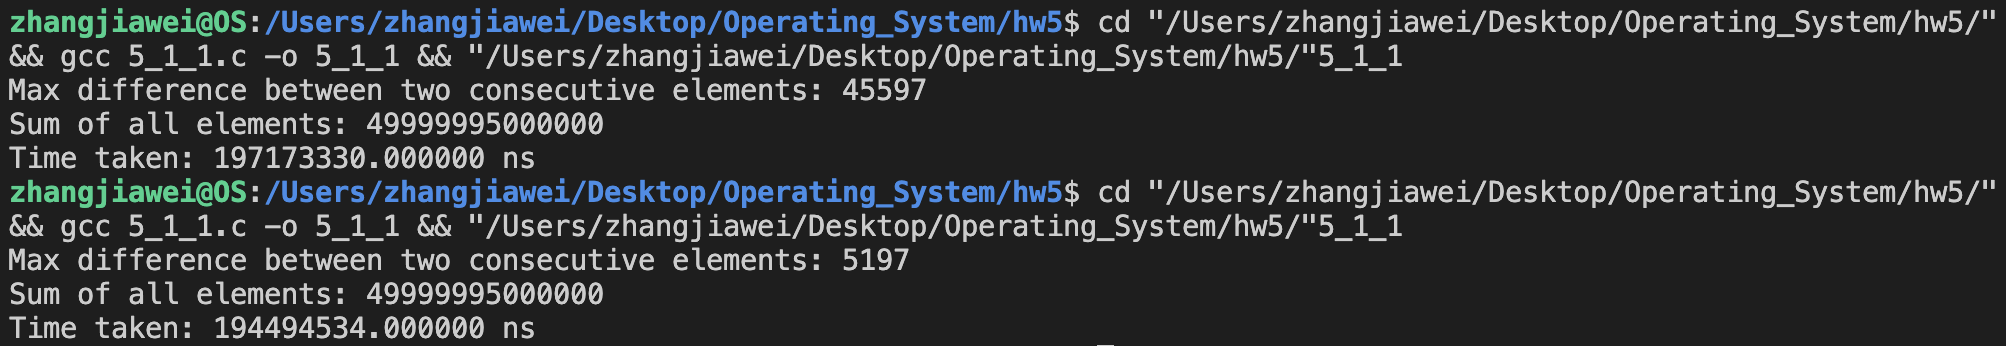
\includegraphics[width=\textwidth]{5_1_1.png}
      \caption{Peterson算法运行结果}
    \end{figure}

    可以看出,Peterson算法算出了最大相邻元素差值和所有元素的和,同时计算了程序运行时间。由元素和得知,程序运行正确,但是最大相邻元素差值具有随机性,这是因为CPU调度的不确定性导致的。

    \item 使用\texttt{pthread_mutex_lock/unlock()}实现互斥访问,代码如下:
    
    \begin{lstlisting}[language=C]
        #include <stdio.h>
        #include <stdlib.h>
        #include <stdbool.h>
        #include <pthread.h>
        #include <time.h>
        #include <unistd.h>
        #define MAX 10000000
        #define max(a, b) ((a) > (b) ? (a) : (b))
        
        int idx = 0;
        int idx_even = 0;
        int idx_odd = 0;
        int data[MAX] = {0};
        pthread_mutex_t mutex = PTHREAD_MUTEX_INITIALIZER;
        
        void *even(void *arg) {
            while (idx < MAX){
                pthread_mutex_lock(&mutex);
                // begin critical section
                int count = 0;
                int i = idx_even;
                while (count < 200 && i < MAX){
                    data[idx] = i;
                    idx++;
                    i+=2;
                    count++;
                }
                idx_even += 400;
                // end critical section
                pthread_mutex_unlock(&mutex); 
            }
            return NULL;
        }
        
        void *odd(void *arg) {
            while (idx < MAX){
                pthread_mutex_lock(&mutex);
                // begin critical section
                int count = 0;
                int i = idx_odd;
                while (count < 200 && i < MAX){
                    data[idx] = i+1;
                    idx++;
                    i+=2;
                    count++;
                }
                idx_odd += 400;
                // end critical section
                pthread_mutex_unlock(&mutex);
            }
            return NULL;
        }
        
        int main() {
            pthread_t t1, t2;
            struct timespec start, end;
            pthread_mutex_init(&mutex, NULL);
            clock_gettime(CLOCK_MONOTONIC, &start);
            pthread_create(&t1, NULL, even, NULL);
            pthread_create(&t2, NULL, odd, NULL);
            pthread_join(t1, NULL);
            pthread_join(t2, NULL);
            clock_gettime(CLOCK_MONOTONIC, &end);
            pthread_mutex_destroy(&mutex);
        
            int max_diff = 0;
            long sum = 0;
            for (int i = 0; i+1 < MAX; i++){
                max_diff = max(max_diff, abs(data[i] - data[i+1]));
            }
            for (int i = 0; i < MAX; i++)
                sum += data[i];    
            
            printf("Max difference between two consecutive elements: %d\n", max_diff);
            printf("Sum of all elements: %ld\n", sum);
            printf("Time taken: %lf ns\n", (end.tv_sec - start.tv_sec) * 1e9 + (end.tv_nsec - start.tv_nsec));
            return 0;
        }
    \end{lstlisting}

    临界区已经在代码中标注,运行结果如下:

    \begin{figure}[H]
      \centering
      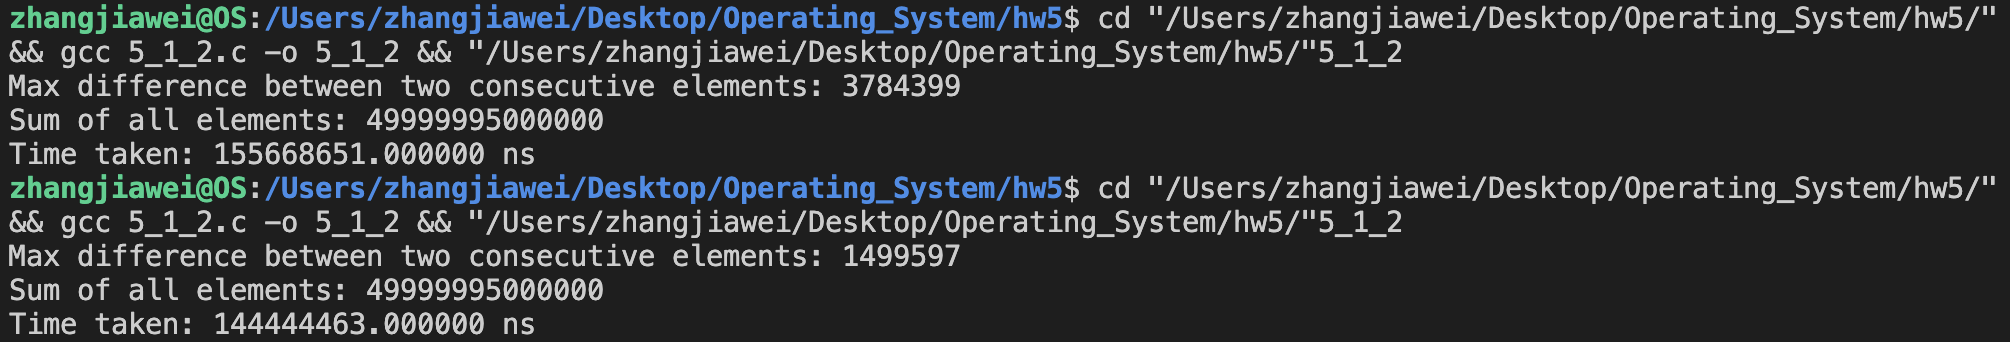
\includegraphics[width=\textwidth]{5_1_2.png}
      \caption{\texttt{pthread\_mutex\_lock/unlock()}运行结果}
    \end{figure}

    与上一题的结果类似,最大相邻元素差值仍因为CPU调度的不确定性而具有随机性,但是元素和的结果表明程序运行正确,运行时间比上一题稍短。

    \item 使用\texttt{atomic_add_fetch}实现互斥访问,代码如下:
    
    \begin{lstlisting}[language=C]
        #include <stdio.h>
        #include <stdlib.h>
        #include <stdbool.h>
        #include <pthread.h>
        #include <time.h>
        #include <unistd.h>
        #include <stdatomic.h>
        
        #define MAX 10000000
        #define max(a, b) ((a) > (b) ? (a) : (b))
        
        atomic_long idx = 0;
        atomic_long idx_even = 0;
        atomic_long idx_odd = 0;
        long data[MAX] = {0};
        
        void *even(void *arg) {
            while (atomic_load(&idx) < MAX) {
                int count = 0;
                long i = atomic_load(&idx_even);
                while (count < 200 && i < MAX) {
                    data[atomic_fetch_add(&idx, 1)] = i;
                    i += 2;
                    count++;
                }
                atomic_fetch_add(&idx_even, 400);
            }
            return NULL;
        }
        
        void *odd(void *arg) {
            while (atomic_load(&idx) < MAX) {
                int count = 0;
                long i = atomic_load(&idx_odd);
                while (count < 200 && i < MAX) {
                    data[atomic_fetch_add(&idx, 1)] = i + 1;
                    i += 2;
                    count++;
                }
                atomic_fetch_add(&idx_odd, 400);
            }
            return NULL;
        }
        
        int main() {
            pthread_t t1, t2;
            struct timespec start, end;
            clock_gettime(CLOCK_MONOTONIC, &start);
            pthread_create(&t1, NULL, even, NULL);
            pthread_create(&t2, NULL, odd, NULL);
            pthread_join(t1, NULL);
            pthread_join(t2, NULL);
            clock_gettime(CLOCK_MONOTONIC, &end);
        
            long max_diff = 0;
            long sum = 0;
            for (int i = 0; i + 1 < MAX; i++) {
                max_diff = max(max_diff, labs(data[i] - data[i + 1]));
            }
            for (int i = 0; i < MAX; i++)
                sum += data[i];
        
            printf("Max difference between two consecutive elements: %ld\n", max_diff);
            printf("Sum of all elements: %ld\n", sum);
            printf("Time taken: %lf ns\n", (end.tv_sec - start.tv_sec) * 1e9 + (end.tv_nsec - start.tv_nsec));
            return 0;
        }
    \end{lstlisting}

    临界区已经在代码中标注,运行结果如下:

    \begin{figure}[H]
      \centering
      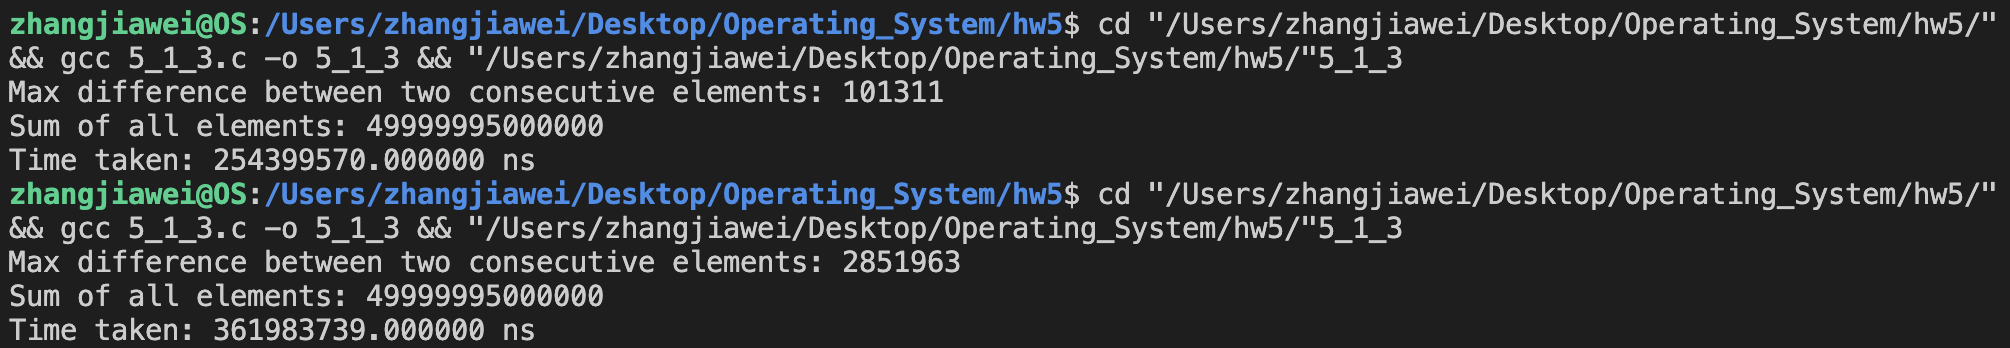
\includegraphics[width=\textwidth]{5_1_3.png}
      \caption{\texttt{atomic\_add\_fetch}运行结果}
    \end{figure}

    本题使用了\texttt{atomic\_add\_fetch}函数实现互斥访问,但是最大相邻元素差值具有随机性,这是因为CPU调度的不确定性导致的。除此之外,在Linux系统下,如果不使用\texttt{long}类型,而是使用\texttt{int}类型,可能会导致溢出,原因未知。
\end{enumerate}

\noindent
\tbf{5.2}

可以实现,代码如下:

\begin{lstlisting}[language=C]
    #include <stdio.h>
    #include <stdlib.h>
    #include <pthread.h>
    #include <time.h>
    #define LEN 5
    #define CYCLE 5
    
    int data[LEN] = {0};
    pthread_mutex_t mutex = PTHREAD_MUTEX_INITIALIZER;
    
    void *randomize(void *arg) {
        struct timespec ts;
        clock_gettime(CLOCK_REALTIME, &ts);
        srand(ts.tv_nsec);
    
        pthread_mutex_lock(&mutex);
        for (int i = 0; i < LEN; i++)
            data[i] = rand() % 20 + 1;
        pthread_mutex_unlock(&mutex);
        return NULL;
    }
    
    void *printArray(void *arg) {
        int sum = 0;
    
        pthread_mutex_lock(&mutex);
        for (int i = 0; i < LEN; i++){
            printf("%d ", data[i]);
            sum += data[i];
        }
        pthread_mutex_unlock(&mutex);
        printf("-> Sum: %d\n", sum);
        return NULL;
    }
    
    int main(){
        pthread_t t1, t2;
        for (int i = 0; i < CYCLE; i++){
            pthread_create(&t1, NULL, randomize, NULL);
            pthread_join(t1, NULL);
            pthread_create(&t2, NULL, printArray, NULL);
            pthread_join(t2, NULL);
        }
        return 0;
    }
\end{lstlisting}

运行结果如下:

\begin{figure}[H]
  \centering
  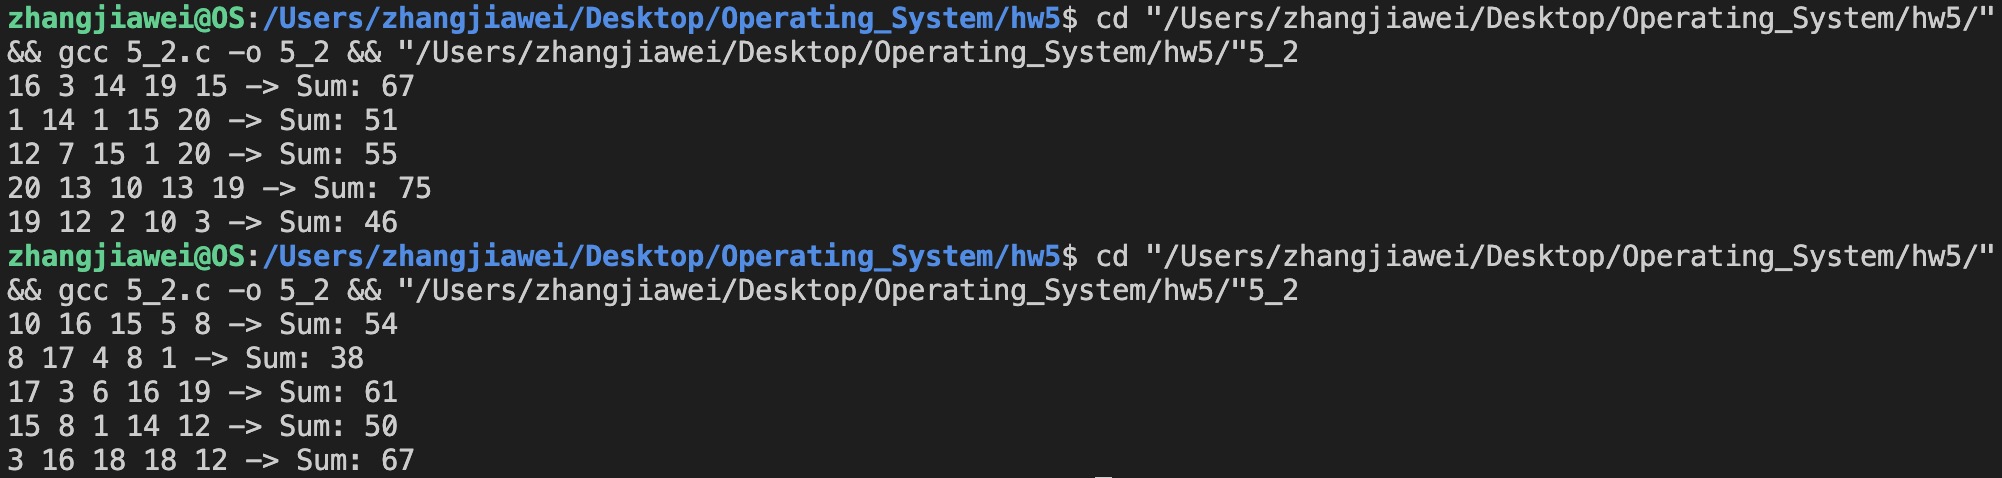
\includegraphics[width=\textwidth]{5_2.png}
  \caption{随机生成数组并打印}
\end{figure}

可以看出,程序成功使用互斥锁实现了随机生成数组并打印的功能,每次生成的数组元素和都不相同。需要注意的是,随机数种子使用了当前时间的纳秒部分,以保证每次生成的随机数不同,若不使用纳秒部分,可能会导致每次生成的随机数相同。
\end{document}